\documentclass{article}
\textheight 23.5cm \textwidth 15.8cm
%\leftskip -1cm
\topmargin -1.5cm \oddsidemargin 0.3cm \evensidemargin -0.3cm
%\documentclass[final]{siamltex}

\usepackage{ctex}
\usepackage{verbatim}
\usepackage{fancyhdr}
\usepackage{graphicx}
\usepackage{amsmath}
\usepackage{amssymb}
\usepackage{float}
\usepackage{multirow}
\usepackage{colortbl}
\usepackage{amsthm}
\usepackage{bm}
\usepackage{tikz}

\textheight 23.5cm \textwidth 15.8cm
\topmargin -1.5cm \oddsidemargin 0.3cm \evensidemargin -0.3cm
\title{HW9 实验报告}
\author{PB20010429 侯相龙}

\begin{document}
\maketitle
\section{实验内容}
用 OpenGL 实现纹理映射

\section{实验原理}

Tutte 均匀参数化后,将纹理映射到$\mathbb{R}^2$参数空间,再将参数空间中的像素值映射到$\mathbb{R}^3$上的曲面。

\section{算法介绍与步骤}
\begin{description}
    \item[1)]作业 5 中参数化结果作为纹理坐标(uv),该坐标已预先保存tutte.txt文件中供主函数读取。
    \item[2)]以 bricks2.jpg 图像作为纹理,给三角网格贴上纹理
\end{description}


\section{测试数据与实验结果}
实验结果如下

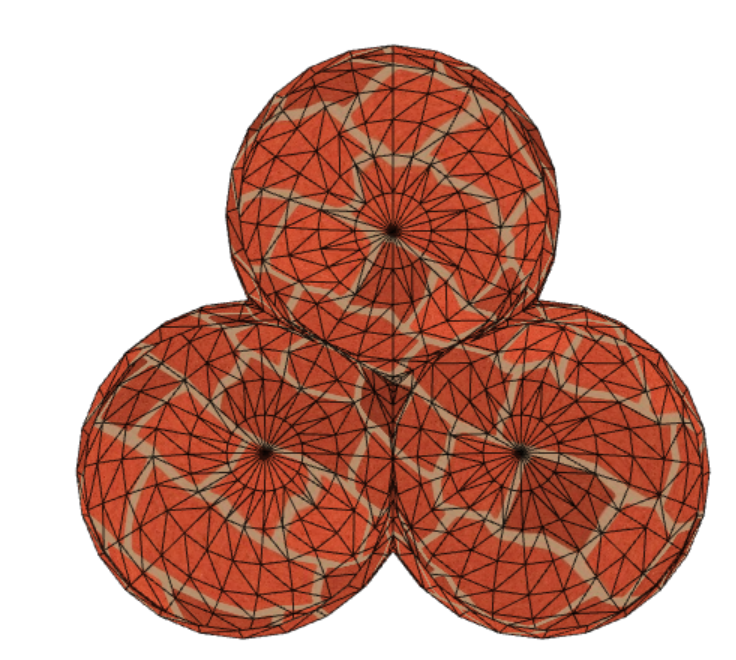
\includegraphics[width=0.5\linewidth]{1.png}
\qquad
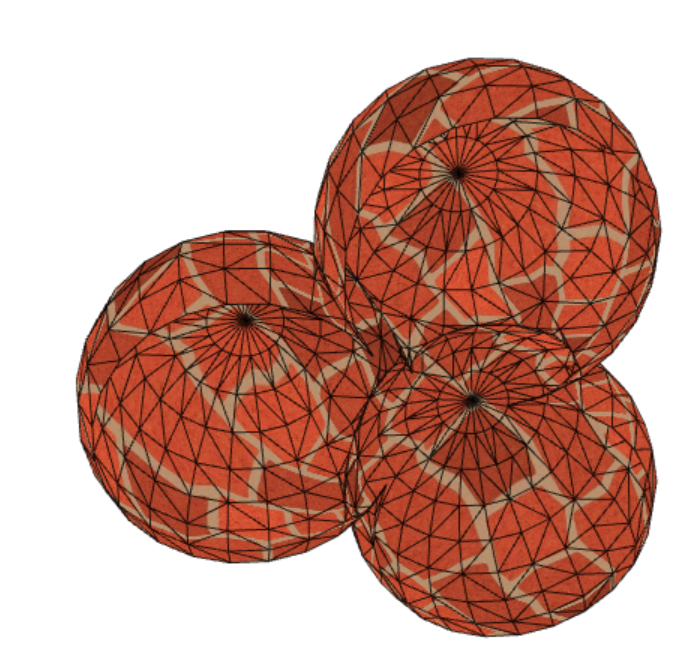
\includegraphics[width=0.5\linewidth]{2.png}




\end{document}
